%Results
%  *rationale for the choice of permeants (Yi, Nelson, Chris T.)
%    -range of expected logPs, experimental data for real membranes (not just PAMPA)
%    -also explores force field reliability (codeine just run through paramchem for example)

\section*{Results and Discussion}
Below, we report the membrane permeability coefficients (\perm) of urea, benzoic acid, and codeine computed with four different methods, namely, US, REUS, ABF and MW-ABF.  We also present a detailed analysis of two methods for the computation of diffusivity, namely, a Bayesian inference method and a Generalized Langevin method. While we did not test metadynamics, another common free-energy method, it has recently been favorably compared with US for water-membrane partitioning, nonetheless while suffering the same shortcomings~\cite{Bochicchio2015}.  Initial states, i.e., positions of the permeant within the bilayer, were generated using 100-ns steered MD simulations~\cite{Izrailev1997,Sotomayor2007} in which the permeant is pulled from one side of the membrane to the other (see Methods).
%We will first compare our results with experimentally measured logP$_{m}$, and then evaluate the performance of different methods in computing the PMFs and diffusivities of various permeants, followed by a discussion on the error and robustness of the four methods.

The three permeants studied here, shown in Fig.~\ref{fig:permeants}, are chosen for their diverse chemical properties:
their molecular weights range from 60\,g/mol (urea) to 299\,g/mol (codeine);
their hydrophilicity, as measured by the octanol:water partition coefficient, differs by over two orders of magnitude;
and most importantly, the experimentally determined \perm~of the three permeants span five orders of magnitude (Table\,1), making them a relatively robust test set for \perm~calculation via different methods. Of the three permeants, benzoic acid is the only permeant that exhibits a formal charge at pH=7. Nonetheless, only its neutral form is considered in our calculation. This treatment is consistent with the corresponding experimental protocol~\cite{Walter1984}, where fluxes at several pH values are measured to determine the `intrinsic permeability' corresponding to the un-ionized form of a given molecule. The underlying assumption of such a protocol, i.e., only the non-ionized form of benzoic acid contributes significantly to \perm, has been confirmed experimentally~\cite{Walter1984}.

\begin{figure}[htbp]
\begin{center}
	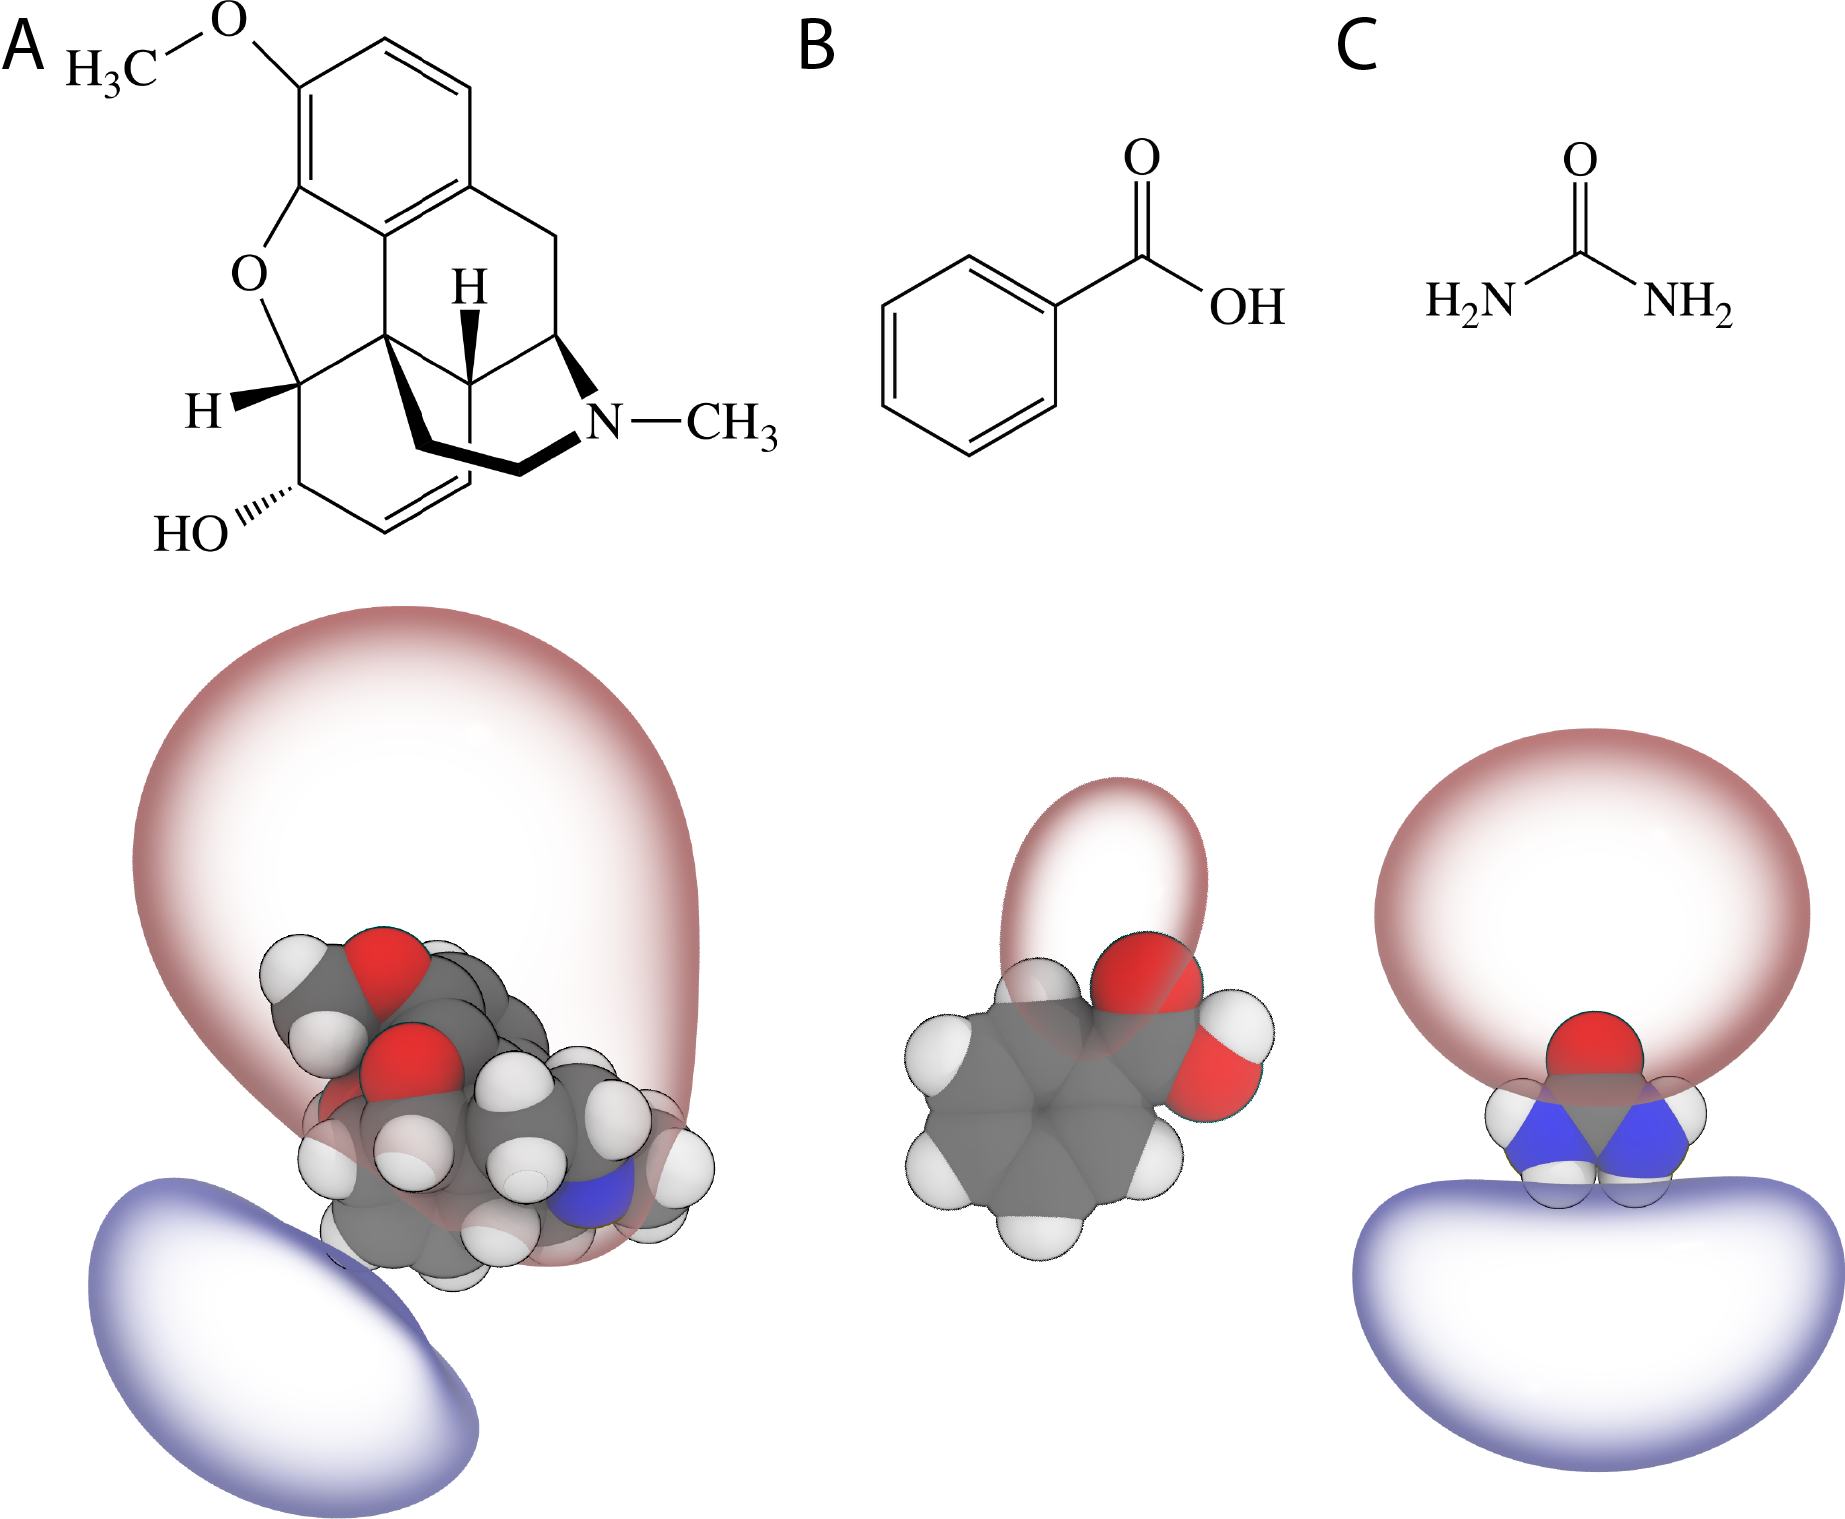
\includegraphics[width=0.6\textwidth]{2015-permeability/Figures/permeants1}
	\caption{Three permeants tested shown as 2D schematics (top) and 3D structures rendered with the $\pm 5$ kT/e electrostatic potential isosurfaces
% JC: What is PME?
% calculated by PME
using the assigned CGenFF charges (bottom).  (A) codeine.  (B) Benzoic acid (neutral).  (C) Urea.}
	\label{fig:permeants}
\end{center}
\end{figure}

%We should add a section about system set up, to include a description of the use of SMD to generate the starting states. This brief section could go here.
% whoops, overlooked this comment; still SMD is now mentioned above
